\documentclass[blockverticalspace=20mm,colspace=20mm,25pt]{tikzposter} %Options for format can be included here
\usepackage{pgfplots}
\usepackage{amsmath}
\usepackage{amsfonts}
\usepackage{amssymb}
%\usepackage{amsthm}
\usepackage{setspace}
\onehalfspacing
\usepackage{graphicx}
\newcommand*{\Scale}[2][4]{\scalebox{#1}{$#2$}}%

\geometry{paperwidth=90cm,paperheight=160cm}

\linespread{1.07}


\usetikzlibrary{arrows,positioning,arrows.meta} 
\tikzset{
    %Define standard arrow tip
    %>=stealth',
    >={Latex[width=5mm,length=7mm]},
    %Define style for boxes
    punkt/.style={
           rectangle,
           rounded corners,
           draw=black, very thick,
           text width=11.5em,
           minimum height=2em,
           text centered},
    % Define arrow style
    pil/.style={
           ->,
           thick,
           shorten <=2pt,
           shorten >=2pt,}
}

%\newtheorem*{mydef}{Definition}
\newtheorem{theorem}{Theorem}

\renewcommand\Re{\mathop{\rm Re}\nolimits}
\renewcommand\Im{\mathop{\rm Im}\nolimits}



 % Title, Author, Institute
\title{
\vbox{
\bf Inverse problems for Sturm-Liouville operators  
with Bessel-type singularity inside an interval
}
}
\author{Alexey Fedoseev}
\institute{Saratov State University, Russia}
%\titlegraphic{LogoGraphic Inserted Here}

 %Choose Layout
%\usetheme{Default}

\usetheme{Board}
%\usetheme{Rays}
%\usecolorstyle{Russia}
\tikzposterlatexaffectionproofoff

\begin{document}


 % Title block with title, author, logo, etc.
%\maketitle[titletoblockverticalspace=7cm]
\maketitle

\begin{columns}

\column{0.5}

\block{\Huge What is Inverse Problem?}{
%\innerblock{}
\Large
Inverse problems are concerned with determining causes for a desired or an observed effect.




\begin{tikzfigure}[A relation between direct and inverse problems]
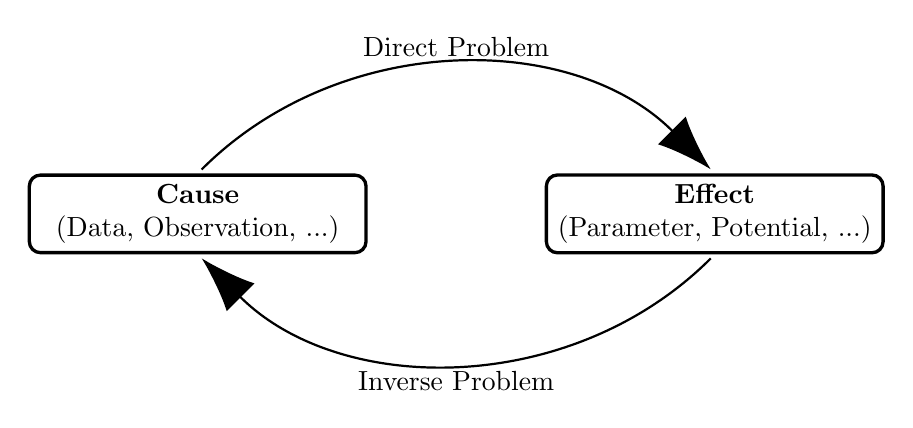
\begin{tikzpicture}[node distance=1cm, auto]
 \node (dummy) {};
 \node[punkt, left = of dummy] (cause) {\textbf{Cause}\\(Data, Observation, ...)};
 \node[punkt,right=of dummy]  (effect) {\textbf{Effect}\\(Parameter, Potential, ...)};
 \draw (cause.north) edge[pil,->, bend left=45] node[auto] {Direct Problem} (effect.north);
 \draw (effect.south) edge[pil,->, bend left=45] node[auto] {Inverse Problem} (cause.south);
\end{tikzpicture}
\end{tikzfigure}




%\innerblock{What is Inverse Problems?}{
%Solution of an inverse problem entails determining unknown causes, based on observation of their effects.
%}
%Solution of an inverse problem entails determining unknown causes, based on observation of their effects.


The situation in which the parameters or sources are directly accessible by measurement is called direct measurement. However, in many cases, the information searched for is not directly measurable. Instead, it is physically connected to other measurable values. We call this situation indirect measurement. 
%Though these measurable values are evidently dependent on the physics of the studied phenomenon, they are also dependent on the measurement instruments employed. 
The laws of physics that link observable information to the values searched for are generally mathematically complex, using, for example, integral equations or partial derivatives. The solution to a problem that calculates observable effects from unknown values, or a direct problem, is often simpler 
%and more easily mastered 
than that of an inverse problem, which calculates unknown values from observable effects.
}


\block{\huge Neptune}{
\Large
The discovery of the planet Neptune is a famous example of an inverse problem. At the beginning of the 19th century, the most distant discovered planet was Uranus. When astronomers applied Newton's theory of universal gravitation to the movement of Uranus, the calculations did not match the observed orbit and movement. 



\begin{tikzfigure}[Neptune]
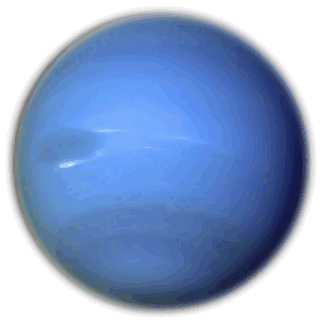
\includegraphics[scale=1.5]{Neptune.pdf}
\end{tikzfigure}



In 1844 a French mathematician Urbain Le Verrier began to labor away at this calculation, using inverse perturbations of features (mass, orbit, current position) of the hypothetical planet assumed to produce Uranus' observed irregularities. In his report to the Academy of Sciences on August 31, 1846, Le Verrier presented the orbital elements of this new planet. Then, on September 23 the Berlin astronomer Galle received from Le Verrier a letter detailing its predicted position and succeeded in observing the object.
}



\block{\huge First Result}{
\Large
The inverse spectral problems theory was discovered and introduced by Soviet-Armenian astrophysicist Victor Ambartsumian.

Just after his graduation from the University of Leningrad he was interested in what degree do the eigenvalues of an ordinary differential operator determine the functions and parameters entering into that operator? Ambartsumian published in 1929 in Zeitschrift f\"ur Physik a paper which contained the statement of the general problem and the proof of the theorem that among all strings the homogeneous string is uniquely defined by the set of its oscillation-frequencies.



\innerblock[titleleft]{\LARGE Theorem}{
Consider the boundary value problem
\begin{equation}
\huge -y''+q(x)y=\lambda y, \quad y'(0)=y'(\pi)=0.
\label{Ambartsumian}
\end{equation}
%Clearly, if $q(x)=0$ a.e. on $(0,\pi),$ then the eigenvalues of \eqref{Ambartsumian} have the form $\lambda_n=n^2$,$n\ge 0$. Ambartsumian proved the inverse assertion:

%\innerblock[titleleft]{Theorem}{
%If the eigenvalues of \eqref{Ambartsumian} are
If the eigenvalues of \eqref{Ambartsumian} are
$\lambda_n=n^2,\;n \ge 0,$ then $q(x)=0$ a.e. on $(0,\pi)$.
}



During the fifteen years nobody has taken notice of that paper. However in 1944 that work was found by Swedish mathematicians who have obtained many interesting results related to the ''inverse Sturm-Liouville problem`` and thus that paper became the foundation of an entire discipline.
}



\block{\refname}{
\small
%[1] Fedoseev A. bla-bla-bla in mechanics. Mega J. 2013
%
%[2] Fedoseev A. bla-bla-bla in mechanics. Mega J. 2013
%
%[3] Fedoseev A. bla-bla-bla in mechanics. Mega J. 2013

{\def\section*#1{}
\begin{thebibliography}{100}
\bibitem{lapwood81} 	
	Lapwood F. R., Usami T., Free Oscillations of the Earth, Cambridge University Press, Cambridge, 1981
\bibitem{const98} 		
	Constantin A., On the inverse spectral problem for the Camassa-Holm equation, J. Funct. Anal., 1998, 155, 352-363	
\bibitem{yurko-freiling-99} 
	Freiling G., Yurko V. A.,  Reconstructing parameters of a medium from incomplete spectral information, Results Math., 1999, 35, 228-249
\bibitem{fedoseev-izvsgu-13}
    Fedoseev A.E. Necessary and Sufficient Conditions for the Solvability of the Inverse Problem for Sturm-Liouville Operators with a Nonintegrable Singularity Inside a Finite Interval, Izv. Saratov. Univ. Mat. Mekh. Inform., vol. 13, num. 3, 2013, 59-64 (in Russian).
\bibitem{fedoseev-cejm-13}
\textbf{Fedoseev A. An inverse problem for Sturm–Liouville operators on the half-line having Bessel-type singularity in an interior point, Cent. Eur. J. Math., vol. 11, num. 12, 2013, 2203-2214.}
\bibitem{fedoseev-izvsgu-12}
    Fedoseev A.E. Inverse problem for Sturm-Liouville operator on the half-line  having nonintegrable singularity, in an interior point, Izv. Saratov. Univ. Mat. Mekh. Inform., vol. 12, num. 4, 2012, 49-55 (in Russian).        
\bibitem{fedoseev-tamkang-11}
\textbf{Fedoseev A. Inverse problems for differential equations on the half-line having a singularity in an interior point, Tamkang J. Math., vol. 42, num. 3, 2011, 343-354.}
    
\end{thebibliography}
}
}

\block{Acknowledgements}{
This work was supported by the Ministry of Education and Science of the
Russian Federation (Grant 1.1436.2014K) and NANUM 2014 Travel Grant.
}

\column{0.5}





%\end{columns}



 %\begin{columns}

 % FIRST column
%\column{0.5}% Width set relative to text width





 




%\block{hghgjhg}{
%\begin{tikzfigure}[A figure can be made withoes not work]
%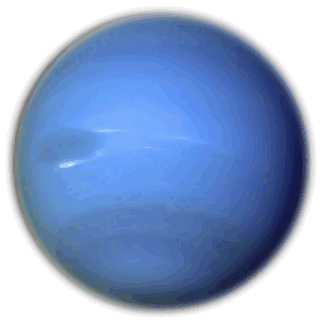
\includegraphics[scale=1]{Neptune.pdf}
%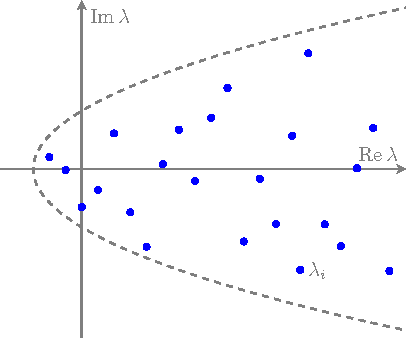
\includegraphics[scale=1]{spectra.pdf}
%\begin{tikzpicture}[scale=1]
%\draw [->, color=gray,thick] (0,0) node[below] {$0$}-- (5,0) node[below] {$x$};
%\node[shape=circle,fill=red,scale=0.3] at (2,0) {};
%\node[below,color=gray] at (2,-0.1) {$a$};
%\end{tikzpicture}
%\end{tikzfigure}
%}

%\block{hgjhgjhgjhg}{
%An interesting kind of generalization of Bessel equation is ...
%It can be easily obtained by taking a substitution...
%}


\block{\huge The Problem}{
\Large
Consider the boundary value problem  ${\cal L=L}(q)$
\begin{equation}
\LARGE
\begin{cases}
-y''+\Big(\dfrac{\nu_0}{(x-a)^2}+q(x)\Big)y=\lambda y,\quad x>0,\\
y(0)=0
\end{cases}
\label{initeq}
\end{equation}
%Consider the differential equation
%\begin{equation}
%\ell y = -y''+\Big(\frac{\nu_0}{(x-a)^2}+q(x)\Big)y=\lambda y,\quad x>0,
%\label{initeq}
%\end{equation}
on the half-line with a Bessel-type singularity at an interior point $a>0$ and an additional \textit{matching conditions} near the singular point $x=a$ (see below). 








Here $q(x)$ is a complex-valued function and $\nu_0$ is a complex number. Let $\nu_0=\nu^2-1/4$ and to be definite, we assume that  $Re\,\nu>0,$ $\nu\neq 1,2,\ldots$ 
%(the other cases require minor modifications). 
We also assume that 
$q(x)|x-~a|^{\min(0,1-2Re\,\nu)} \in L(0,T)$ for some $T>a$ and $q(x)\in L(T,\infty)$. 
%\[
%q(x)|x-~a|^{\min(0,1-2Re\,\nu)} \in L(0,T) \text{ for some } T>a \text{ and } q(x)\in L(T,\infty). 
%\]

\begin{tikzfigure}[$a\in(0,\infty)$]
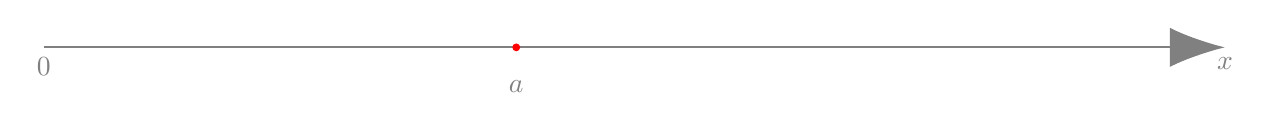
\begin{tikzpicture}[scale=3]
\draw [->, color=gray,thick] (0,0) node[below] {$0$}-- (5,0) node[below] {$x$};
\node[shape=circle,fill=red,scale=0.3] at (2,0) {};
\node[below,color=gray] at (2,-0.1) {$a$};
\end{tikzpicture}
\end{tikzfigure}

%We denote the class of such functions $q(x)$ by $W$.

%The paper deals with the boundary value problem  ${\cal L=L}(q)$ for differential equation \eqref{initeq} with the Dirichlet boundary condition $y(0)=0$ and an additional \textit{matching conditions} near the singular point $x=a$. 
%We consider in some sense arbitrary matching conditions with a transition matrix $A=[a_{jk}]_{j,k=1,2},$ that connects solutions of \eqref{initeq} in a neighborhood of the singular point. 

Inverse problems for differential equations with singularities inside an 
interval are important in mathematics and its applications. A wide class of differential
equations with turning points can be reduced to equations with singularities. For example, inverse
problems for such equations occur in electronic engineering in designing heterogeneous transmission
channels with given characteristics \cite{yurko-freiling-99}. Boundary value problems with a discontinuity at an interior
point also arise in geophysical models of the Earth's crust \cite{lapwood81}. Inverse problems for equations
with singularities and turning points are used in investigations of the discontinuous solutions of
some integrable nonlinear equations of mathematical physics \cite{const98}. 
%Note that in different problems of natural sciences, various matching conditions for solutions with the corresponding transition matrices $A$ are used.

}




%\column{0.5}
 %Second column with first block's top edge aligned with with previous column's top.
\block{\huge Matching Conditions}{
\Large
We consider in some sense arbitrary matching conditions with a transition matrix $A=[a_{jk}]_{j,k=1,2},$ that connects solutions of \eqref{initeq} in a neighborhood of the singular point. 

Let $\lambda=\rho^2$ and $\mathrm{Im}\,\rho\geq0$. Consider the functions
\[
C_j(x,\lambda)=(x-a)^{\mu_j} \sum^\infty_{k=0} c_{jk}(\rho (x-a))^{2k} ,\; j=1,2,
\]
where $c_{10}c_{20}=(2\nu)^{-1}$,
\[
\mu_j=(-1)^j\nu+1/2,\, c_{jk}=(-1)^k c_{j0}
\,\Big( \prod^k_{s=1} ((2s+\mu_j)(2s+\mu_j-1)-\nu_0)\Big)^{-1}.
\]
Here 
%and below 
$z^{\mu}=\exp(\mu(\mbox{ln}|z|+i\arg z))$, $\arg z \in (-\pi, \pi]$. If $x>a$ or $x<a$ then the functions
 $C_j(x,\lambda)$ are solutions of \eqref{initeq} with $q(x)\equiv 0$. Let the functions $s_j(x,\lambda)$, $j=1,2$ be solutions of the following integral equations for $x>a$ and $x<a$: 
\[
s_j(x,\lambda)=C_j(x,\lambda)+\int^x_{a} g(x,t,\lambda)q(t)s_j(t,\lambda)\,dt,
\]
where $g(x,t,\lambda)=C_1(t,\lambda)C_2(x,\lambda)-C_1(x,\lambda)C_2(t,\lambda)$. For each fixed $x$ the functions $s_j(x,\lambda)$ are entire in $\lambda$ of order 1/2 and form a fundamental system of solutions of \eqref{initeq}. 
%Moreover 
%\begin{equation}
%\det[s_j^{(m-1)}(x,\lambda)]_{j,m=\overline{1,2}}\equiv 1. 
%\label{detsj}        
%\end{equation} 

%Let $A=[a_{jk}]_{j,k=1,2}$, $\det A\ne 0$ be a given matrix with complex numbers $a_{jk}$. We introduce the functions  $\{\sigma_j(x,\lambda)\}_{j=1,2}$, $x\in J_{-}\cup J_{+}$, $J_{\pm}=\{\pm (x-a)>0\}$ by the formula
Let $A=[a_{jk}]_{j,k=1,2}$, $\det A\ne 0$ be a given matrix with complex numbers $a_{jk}$. We introduce the functions  $\{\sigma_j(x,\lambda)\}_{j=1,2}$, $x\neq a$ by the formula
\begin{equation*}
\sigma_j(x,\lambda)=
\begin{cases}
s_j(x,\lambda), & x<a,\\
\sum\limits_{k=1}^{2}a_{kj}s_k(x,\lambda),&  x>a.
\end{cases}
\label{sigmajinsk}
\end{equation*}
The fundamental system of solutions $\{\sigma_j(x,\lambda)\}$ is used to match solutions in a neighborhood of the singular point  $x=a$. 
%It follows from \eqref{detsj} that
%\begin{equation}
%\det[\sigma_j^{(m-1)}(x,\lambda)]_{j,m=1,2}\equiv
%\left\{ \begin{array}{ll}
%1,\quad & x\in J_{-}, \\ \det A,\quad & x\in J_{+}.
%\end{array}\right. 
%\label{detsigmaj}                
%\end{equation}

%We introduce numbers $\xi_{jk}$, $j,k=1,2$ by
%\begin{equation}
%\left[ \begin{array}{ll}
%\xi_{11} & \xi_{12} \\ \xi_{21} & \xi_{22}
%\end{array}\right]= \frac{1}{2\sin\pi\nu}
%\left[ \begin{array}{ll}
%-a_{11}e^{2\pi i\nu}+a_{22}e^{-2\pi i\nu} & -i(a_{11}e^{\pi i\nu}-a_{22}e^{-\pi i\nu}) \\
%-i(a_{11}e^{\pi i\nu}-a_{22}e^{-\pi i\nu}) & a_{11}-a_{22} 
%\end{array}\right] .    
%\label{ksimatrix}
%\end{equation}       
%The behaviour of the spectrum of the boundary value problem ${\cal L}$ depends on the numbers $\xi_{jk}$. 
We consider the most difficult special case when
%$|\xi_{jj}|>|\xi_{12}|>0$, since in this case 
the discrete spectrum is unbounded and essential qualitative modifications in the investigation of the direct and inverse problems are arised. 
%To be definite we set $a_{12}=0$ (the other case requires minor modifications).
\begin{tikzfigure}[The spectrum of boundary value problem {\cal L}.]
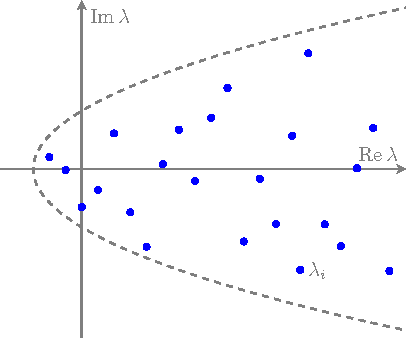
\includegraphics[scale=2]{spectra.pdf}
\end{tikzfigure}
}

%\block{Using Method of Spectral Mappings}{
%\innerblock[titleleft]{Uniqueness Theorem}{
%%If $M(\lambda)=\widetilde M(\lambda)$, then $q(x)=\tilde q(x)$ almost everywhere for $x>0$. Thus, the Weyl function uniquely determines the boundary value problem $\cal L$.
%The Weyl function uniquely determines the boundary value problem $\cal L$.
%}
%}

\block{\huge The Inverse Problem}{
\Large
Let the function $\Phi(x,\lambda)$ be a solution of \eqref{initeq} under conditions
\[\Scale[1.3]{\Phi(0,\lambda)=1, \quad\Phi(x,\lambda)=O(e^{i\rho x}),\quad x\to\infty.}\]
%\begin{equation*}
%\Phi(0,\lambda)=1, \quad\Phi(x,\lambda)=O(e^{i\rho x}),\quad x\to\infty.
%%\quad \rho\in\Omega.
%\end{equation*}
where $\Im\rho\geq0$, $\rho\neq0$.
%WHAT IS ${\cal L}$??????
%$\Phi(0,\lambda)=1$, $\Phi(x,\lambda)=O(\exp(i\rho x))$, $x\to\infty$, $\rho\in\Omega$. 
%\innerblock{}
{
%Function $\Phi(x,\lambda)$ is called the \textit{Weyl solution} for ${\cal L}$.
%Function $\Phi(x,\lambda)$ is called the \textit{Weyl solution} for the problem \eqref{initeq}.
}
%\innerblock{}
{
%The function $M(\lambda):=\Phi'(0,\lambda)$ is called the {\it Weyl function} for ${\cal L}$.

The function 
\[\Scale[1.3]{M(\lambda):=\Phi'(0,\lambda)}\]
is called the {\it Weyl function} for the problem \eqref{initeq}.
}

\

\innerblock[titleleft]{Inverse Problem}{
Recover $q(x)$ by the given Weyl function $M(\lambda)$.
}

\

\innerblock[titleleft]{Uniqueness Theorem}{
%If $M(\lambda)=\widetilde M(\lambda)$, then $q(x)=\tilde q(x)$ almost everywhere for $x>0$. Thus, the Weyl function uniquely determines the boundary value problem $\cal L$.
%The Weyl function uniquely determines the boundary value problem $\cal L$.
The Weyl function uniquely determines the boundary value problem \eqref{initeq}.
}

}





 \end{columns}


\end{document}


\endinput
%%
%% End of file `tikzposter-template.tex'.
